\documentclass[compress,beamer,aspectratio=169,english,usenames,dvipsnames]{beamer}

\usetheme{Singapore}

% Packages
\usepackage[english]{babel} % Set document language
\usepackage{pdfpages} % Include PDF files
\usepackage[utf8]{inputenc} % UTF-8 encoding (for umlauts etc.)
\usepackage[T1]{fontenc} % correct hyphenation
\usepackage{csquotes} % correct quotation marks
\usepackage{lmodern} % Computer Modern fonts
\usepackage{microtype} % better typesetting results (avoids underfull / overfull hboxes)
\usepackage{graphicx} % adding graphics
\usepackage{units} % typesetting units, e.g., \unit[10]{MB} and \unitfrac[100]{Mbit}{s}
\usepackage{booktabs} % publication quality tables
\usepackage{setspace} % Set line spacing
\usepackage{geometry} % Set page margins
\usepackage{subcaption} % Subfigures
\usepackage{float} % Floats
\usepackage[
	backend=biber,
	style=authoryear,
	doi=false,
	url=false,
	maxcitenames=1,
	uniquelist=false
]{biblatex} % Bibliography
\usepackage{hyperref} % Hyperlinks
\usepackage[super]{nth} % Superscript for numbers
\usepackage{amsmath} % Math symbols
\usepackage{amssymb} % Math symbols
\usepackage{mathtools} % Math symbols
\usepackage{amsthm} % Math symbols
\usepackage{bm} % Bold math symbols
\usepackage{tikz} % Drawing
\usepackage{tikz-qtree} % Drawing trees
\usepackage{etoolbox} % Patching
\usepackage{multicol} % Multiple columns
\usepackage{accents} % Math accentsdef
\usepackage[normalem]{ulem} % Underlining
\usepackage{etoolbox} % Patching
\usepackage{listings} % Code listings
\usepackage{bbm} % Blackboard bold

% Custom Definitions
% Functions &
\newcommand{\polyhedron}[1]{\mathcal{#1}}
\newcommand{\mat}[1]{{\bm{#1}}}
\renewcommand{\vec}[1]{{\bm{#1}}}
\newcommand{\conv}[0]{\operatorname{conv}}
\newcommand{\raycone}[0]{\operatorname{cone}}
\newcommand{\transpose}[0]{^\intercal}
\renewcommand{\setminus}{\backslash}
\newcommand{\rank}[0]{\operatorname{rank}}
\newcommand{\st}[0]{\operatorname{s.t.}}
\newcommand{\LP}[0]{\textit{LP}}
\newcommand{\DP}[0]{\textit{DP}}
\newcommand{\IP}[0]{{\textit{IP}}}
\newcommand{\MIP}[0]{\textit{MIP}}
\newcommand{\MP}[0]{{\textit{MP}}}
\newcommand{\LR}[1]{\textit{LR}\ifstrempty{#1}{}{\left({#1}\right)}}
\newcommand{\LDP}[0]{\textit{LDP}}
\newcommand{\RMP}[0]{\textit{RMP}}
\newcommand{\SP}[1]{{\textit{SP}\ifstrempty{#1}{}{^{#1}}}}
\newcommand{\RCP}[0]{\textit{RCP-SP}}
\newcommand{\FP}[0]{\textit{FP-SP}}
\newcommand{\SCIP}[0]{\texttt{SCIP}}
\newcommand{\GCG}[0]{\texttt{GCG}}
\newcommand{\indexset}[1]{\mathcal{#1}}

% Math %

\DeclarePairedDelimiter\abs{\lvert}{\rvert}%
\DeclarePairedDelimiter\norm{\lVert}{\rVert}%
\DeclarePairedDelimiter\floor{\lfloor}{\rfloor}
\DeclarePairedDelimiter\ceil{\lceil}{\rceil}

% Swap the definition of \abs* and \norm*, so that \abs
% and \norm resizes the size of the brackets, and the
% starred version does not.
\makeatletter
\let\oldabs\abs
\def\abs{\@ifstar{\oldabs}{\oldabs*}}
%
\let\oldnorm\norm
\def\norm{\@ifstar{\oldnorm}{\oldnorm*}}
\makeatother

\let\oldbar\bar
\newcommand{\ubar}[1]{{\underaccent{\oldbar}{#1}}}
\renewcommand{\bar}[1]{{\oldbar{#1}}}
\newcommand{\stkout}[1]{\ifmmode\text{\sout{\ensuremath{#1}}}\else\sout{#1}\fi}


% Literature
\addbibresource{literature.bib}
\setbeamertemplate{bibliography item}{}
\usepackage{xpatch}
\xpatchbibmacro{name:andothers}{%
  \bibstring{andothers}%
}{%
  \bibstring[\emph]{andothers}%
}{}{}
\renewbibmacro{in:}{}

\DeclareDocumentCommand\courseTitle{}{Component Bound Branching in a Branch-and-Price Framework}
\DeclareDocumentCommand\exerciseSpeakerName{}{Til Mohr}
\DeclareDocumentCommand\exerciseSpeakerMail{}{\email{til.mohr@rwth-aachen.de}}
\DeclareDocumentCommand\exerciseTopic{}{}


\title{\courseTitle}
\author{Til Mohr}


\begin{document}

\begin{frame}[plain]
\title{\courseTitle}
\subtitle{\exerciseTopic}
\author{\textbf{Til Mohr}\newline
	\url{til.mohr@rwth-aachen.de}\smallskip\smallskip\newline
	%
	Master thesis at the \newline
	Chair of Operations Research @ RWTH Aachen\newline
	\url{www.or.rwth-aachen.de}\smallskip\newline
	%
}
\date{September 19, 2024}
\titlepage
\end{frame}

\nocite{*}

\section{Introduction}
\begin{frame}
\frametitle{Dantzig-Wolfe Reformulation for \IP{}s}
\begin{itemize}
\item	consider the following bounded integer program (\IP{}):
		\begin{equation*}
		\begin{aligned}
		z^*_\IP{} = &\min & \mat{c}\transpose \mat{x} & & & \\
		&\st & \mat{A} \mat{x} & \geq \mat{b} & \left[\mat{\pi}_\mat{b}\right] & \\
		&& \mat{D} \mat{x} & \geq \mat{d} & \left[\mat{\pi}_\mat{d}\right] & \\
		&& \mat{x} & \in \mathbb{Z}_ +^n
		\end{aligned}
		\end{equation*}
\item	we want to solve this \IP{} using Column Generation (CG)
\pause
\item[$\rightarrow$]	Apply Dantzig-Wolfe Reformulation
\end{itemize}
\end{frame}

\begin{frame}
\frametitle{Dantzig-Wolfe Reformulation for \IP{}s}

\begin{itemize}
\item	reformulation using discretization yields the master problem (\MP{}):
		\begin{equation*}
		\begin{aligned}
		z^*_\MP{} = &\min & \sum_{q \in Q} c_q \lambda_q & & & \\
		&\st & \sum_{q \in Q} \mat{a}_q \lambda_q & \geq \mat{b} & \left[\mat{\pi}_\mat{b}\right] \\
		&& \sum_{q \in Q} \lambda_q & = 1 & \left[\pi_0 \right] & \\
		&& \lambda_q & \in \{0, 1\} & & \forall q \in Q
		\end{aligned}
		\end{equation*}
\item	and the subproblem (\SP{}):
		\begin{equation*}
		\begin{aligned}
		z^*_\SP{} = &\min & \left( \mat{c}\transpose - \mat{\pi}_\mat{b}\transpose \mat{A} \right) \mat{x} - \pi_0 & & \\
		&\st & \mat{D} \mat{x} & \geq \mat{d} & \left[\mat{\pi}_\mat{d}\right] \\
		&& \mat{x} & \in \mathbb{Z}_+^n
		\end{aligned}
		\end{equation*}
\end{itemize}
\end{frame}

\begin{frame}
\frametitle{Branch-and-Price}
Branch-and-Price Algorithm:
\begin{enumerate}
\item solve the relaxed \MP{} using CG to optimality
\item branch, if $\vec{\lambda}^*$ is fractional
\item repeat
\end{enumerate}

\vspace{1em}

\pause
But how to branch?
\begin{itemize}
\item	branching on a single $\lambda_q$ is unbalanced:\\$\lambda_q \leq 0$ forbids almost nothing, $\lambda_q \geq 1$ forbids much
\pause
\item[$\rightarrow$]	branch on a set of columns $Q' \subset Q$, such that:
		\begin{equation*}
		\sum_{q \in Q'} \lambda_q^* \eqqcolon K \not\in \mathbb{Z}
		\end{equation*}
\end{itemize}
\end{frame}

\begin{frame}
\frametitle{Component Bound Sequences - \cite{vanderbeck1996exact}}
\begin{itemize}
\item	to find such a set $Q'$ of columns, we find a component bound sequence:
		\begin{equation*}
		S \coloneqq \{ \left( x_i, \eta_i, v_i \right) \mid \eta_i \in \{\leq, \geq\}, v_i \in \mathbb{Z} \}
		\end{equation*}
\pause
\item	a master variable $\lambda_q$ satisfies a component bound $\left( x_i, \eta_i, v_i \right)$ if:
		\begin{equation*}
		x_{q,i} \; \eta_i \; v_i
		\end{equation*}
\item	we define $Q'$ as the set of columns, that satisfy all component bounds in $S$
\item	there always exists a component bound sequence $S$ such that:
		\begin{equation*}
		\sum_{q \in Q'} \lambda_q^* \in \left(0, 1\right)
		\end{equation*}
\end{itemize}
\end{frame}

\begin{frame}
\frametitle{Component Bound Sequences}
\begin{columns}
\begin{column}{0.5\textwidth}
\begin{tabular}{c||c|c|c|c}
 & $q_1$ & $q_2$ & $q_3$ & $q_4$ \\
\hline\hline
$x_{1,q_i}$ & 1 & 1 & 2 & 2 \\
$x_{2,q_i}$ & 1 & 2 & 1 & 2 \\
\hline\hline
$\lambda^*_{q_i}$ & 0.25 & 0 & 0.5 & 0.25 \\
\end{tabular}
\end{column}
\begin{column}{0.5\textwidth}
\pause
\begin{itemize}
\item	Find $S = \{ \left( x_1, \leq, 1 \right) \}$
\item	$Q' = \{ q_1, q_2 \}$
\item 	$\sum_{q \in Q'} \lambda_q^* = 0.25 \not\in \mathbb{Z}$
\end{itemize}
\end{column}
\end{columns}
\end{frame}

\section{Vanderbeck's Generic Branching}

\begin{frame}<beamer>
\frametitle{Table of Contents}
\tableofcontents[currentsection]
\end{frame}

\begin{frame}
\frametitle{Vanderbeck's Generic Branching Scheme - \cite{vanderbeck2011branching}}
\begin{columns}
\begin{column}{0.5\textwidth}
	\centering
	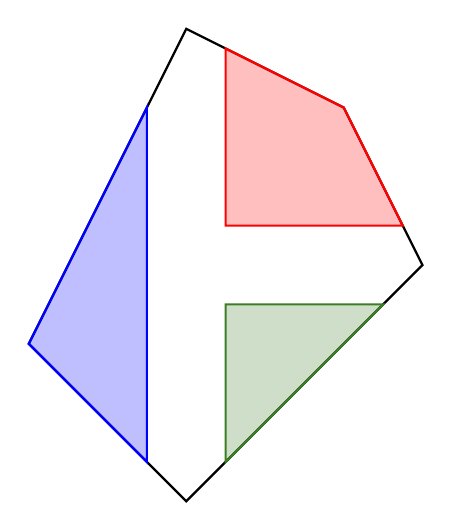
\begin{tikzpicture}
		% Define the coordinates of the polygon
		\coordinate (A) at (0,0);
		\coordinate (B) at (2,4);
		\coordinate (C) at (4,3);
		\coordinate (D) at (5,1);
		\coordinate (E) at (2,-2);

		% Draw the black 5-cornered polygon
		\draw[thick] (A) -- (B) -- (C) -- (D) -- (E) -- cycle;

		% Define the red area coordinates
		\coordinate (R1) at (2.5,3.75);
		\coordinate (R2) at (4,3);
		\coordinate (R3) at (4.75,1.5);
		\coordinate (R4) at (2.5,1.5);
		% Draw the red area with medium transparency
		\fill[red, opacity=0.25] (R1) -- (R2) -- (R3) -- (R4) -- cycle;
		% Outline the red area
		\draw[red, thick] (R1) -- (R2) -- (R3) -- (R4) -- cycle;

		\only<2->{
			% Define the blue area coordinates
			\coordinate (B1) at (0,0);
			\coordinate (B2) at (1.5,3);
			\coordinate (B3) at (1.5,-1.5);
			% Draw the blue area with medium transparency
			\fill[blue, opacity=0.25] (B1) -- (B2) -- (B3) -- cycle;
			% Outline the blue area
			\draw[blue, thick] (B1) -- (B2) -- (B3) -- cycle;

			% Define the green area coordinates
			\coordinate (G1) at (2.5,0.5);
			\coordinate (G2) at (4.5,0.5);
			\coordinate (G3) at (2.5,-1.5);
			% Draw the green area with medium transparency
			\fill[OliveGreen, opacity=0.25] (G1) -- (G2) -- (G3) -- cycle;
			% Outline the green area
			\draw[OliveGreen, thick] (G1) -- (G2) -- (G3) -- cycle;
		}
	\end{tikzpicture}
\end{column}
\begin{column}{0.5\textwidth}
	\begin{itemize}
	\item	assume we have found a component bound sequence\\
			${\color{red} S = \{ \left( x_1, \geq, 1 \right), \left( x_2, \geq, 2 \right) \}}$
	\pause
	\vspace{0.5em}
	\item	create $\abs{S} + 1 = 3$ child nodes:
			\begin{enumerate}
			\item	${\color{blue} S_1 \coloneqq \{ \left( x_1, \leq, 0 \right) \}}$
			\item	${\color{OliveGreen} S_2 \coloneqq \{ \left( x_1, \geq, 1 \right), \left( x_2, \leq, 1 \right) \}}$
			\item	${\color{red} S_3 \coloneqq \{ \left( x_1, \geq, 1 \right), \left( x_2, \geq, 2 \right) \}}$
			\end{enumerate}
	\vspace{0.5em}
	\item	search for solutions only within these regions
	\pause
	\item	refine the regions in deeper nodes
	\end{itemize}
\end{column}
\end{columns}
\end{frame}

\begin{frame}
\frametitle{Enforcing a Component Bound Sequence $S_j$ in Node $j$}
\begin{itemize}
\item	to the \MP{} add constraint:
		\begin{equation*}
		\sum_{q \in Q'_j} \lambda_q \geq 1
		\end{equation*}
\item	move the bounds in the \SP{}:
		\begin{equation*}
		\begin{aligned}
		x_i & \geq v_i & \forall \left( x_i, \geq, v_i \right) \in S_j \\
		x_i & \leq v_i & \forall \left( x_i, \leq, v_i \right) \in S_j \\
		\end{aligned}
		\end{equation*}
\end{itemize}
\end{frame}

\section{Component Bound Branching Rule}

\begin{frame}
\frametitle{Component Bound Branching Rule - \cite{thebook}}
Again:
\begin{itemize}
\item	find a subset $Q'$ of columns using a component bound sequence $S$:
		\begin{equation*}
		S \coloneqq \{ \left( x_i, \eta_i, v_i \right) \mid \eta_i \in \{\leq, \geq\}, v_i \in \mathbb{Z} \}
		\end{equation*}
\item	such that: \quad $\sum_{q \in Q'} \lambda_q^* \in \left(0, 1\right)$
\end{itemize}

\pause

Alternative scheme:
\begin{itemize}
\item	create binary search tree:
		\begin{multicols}{2}
		\noindent
		\begin{minipage}{\linewidth}
		\setlength{\belowdisplayskip}{0pt} \setlength{\belowdisplayshortskip}{0pt}
		\setlength{\abovedisplayskip}{0pt} \setlength{\abovedisplayshortskip}{0pt}
		\begin{equation*}
		\sum_{q \in Q'} \lambda_q \leq 0 \quad \left[\gamma\right]
		\end{equation*}
		\end{minipage}

		\columnbreak

		\noindent
		\begin{minipage}{\linewidth}
		\setlength{\belowdisplayskip}{0pt} \setlength{\belowdisplayshortskip}{0pt}
		\setlength{\abovedisplayskip}{0pt} \setlength{\abovedisplayshortskip}{0pt}
		\begin{equation}
		\sum_{q \in Q'} \lambda_q \geq 1 \quad \left[\gamma\right]
		\end{equation}
		\end{minipage}
		\end{multicols}
\pause
\item	allows for solutions violating $S$ to be found / generated
\end{itemize}
\end{frame}

\begin{frame}
\frametitle{Component Bound Branching Rule - \cite{thebook}}

\begin{itemize}
\item	\SP{} determines whether a new column is in $Q'$, i.e., satisfies $S$
\item	create new variable $y \in \{0, 1\}$ along new constraints, such that: $y = 1 \Leftrightarrow \vec{x} \in S$
\end{itemize}

\pause

\begin{equation*}
\begin{aligned}
z^*_\SP{} = &\min & \left( \mat{c}\transpose - \mat{\pi}_\mat{b}\transpose \mat{A} \right) \mat{x} {\color{blue} - \gamma y} - \pi_0 & & \\
&\st & \mat{D} \mat{x} & \geq \mat{d} & \\
&& {\color{blue} y = 1} &{\color{blue} \Leftrightarrow \sum_{i \in S} y_i = \abs{S}} & \\
&& {\color{blue} y_i = 1} &{\color{blue} \Leftrightarrow x_i \leq v_i }& {\color{blue} \forall \left( x_i, \leq, v_i \right) \in S} \\
&& {\color{blue} y_i = 1} &{\color{blue} \Leftrightarrow x_i \geq v_i }& {\color{blue} \forall \left( x_i, \geq, v_i \right) \in S} \\
&& {\color{blue} y} &{\color{blue} \in \{0, 1\}} & \\
&& {\color{blue} y_i} &{\color{blue} \in \{0, 1\}} & {\color{blue} \forall \left( x_i, \eta_i, v_i \right) \in S} \\
&& \mat{x} & \in \mathbb{Z}_+^n
\end{aligned}
	\end{equation*}
\end{frame}

\begin{frame}
\frametitle{Differences}
\begin{tabular}{c|c}
Vanderbeck's Generic Branching & Component Bound Branching \\
\hline\hline
tightens bounds in \SP{} & adds new variables and constraints to \SP{} \\
$\rightarrow$ use special algorithms & $\rightarrow$ fall back to \MIP{} solver
\pause
\\
\hline
refines component bounds & does not refine component bounds \\
$\rightarrow$ \SP{} becomes faster to solve & $\rightarrow$ \SP{} becomes slower to solve
\end{tabular}
\end{frame}

\section{Generic Mastercuts}

\begin{frame}
\frametitle{Master Constraints without Original Formulation}

\begin{itemize}
\item	we want to add constraint \MP{}:
		\begin{equation*}
		\sum_{p \in P} \operatorname{f}(p) \lambda_p + \sum_{r \in R} \operatorname{f}(r) \lambda_r \leq f \qquad \left[\gamma\right]
		\end{equation*}
\item	with the following modification to the pricing problem:
		\begin{equation*}
		\begin{aligned}
		z^*_\SP{} = &\min & \left( \mat{c}\transpose - \mat{\pi}_\mat{b}\transpose \mat{A} \right) \mat{x} {\color{blue} -\gamma y} - \pi_0 & & \\
		&\st & \mat{D} \mat{x} & \geq \mat{d} & \left[\mat{\pi}_\mat{d}\right] \\
		&& {\color{blue} y} & {\color{blue} = \operatorname{f}(\mat{x})} & \\
		&& \mat{x} & \in \mathbb{Z}_+^n \\
		&& {\color{blue} y} & {\color{blue} \in Y}
		\end{aligned}
		\end{equation*}
\end{itemize}
\end{frame}

\section{Evaluation}

\begin{frame}
\frametitle{Core Evaluation Questions}


\begin{itemize}
\item	implemented generic mastercuts as a new interface in \GCG{}, \cite{gamrath2010generic}
\item	implemented component bound branching using this interface
\end{itemize}
\vspace{1em}
\pause
\begin{enumerate}
\item	Vanderbeck's Generic Branching vs. Component Bound Branching Rule
\item	Dual Value Stabilization: Root-Only vs. Full-Tree
\end{enumerate}
\vspace{1em}
\pause
\begin{itemize}
\item	extracted 736 instances from the structured Integer Programming Library (\texttt{strIPlib}), \cite{strIPlib}
\end{itemize}
\end{frame}

\begin{frame}
\frametitle{Evaluation $\cdot$ Solving Status}
\centering
\begin{figure}
\includegraphics[height=0.85\textheight]{graphics/slides/general/MostFractional/solve_status.png}
\end{figure}
\end{frame}

\begin{frame}
\frametitle{Evaluation $\cdot$ Solving Times}
\centering
\begin{figure}
\includegraphics[height=0.85\textheight]{graphics/slides/general/MostFractional/times.png}
\end{figure}
\end{frame}

\begin{frame}
\frametitle{Evaluation $\cdot$ Outperformance Rate over \texttt{generic}}
\centering
\begin{figure}
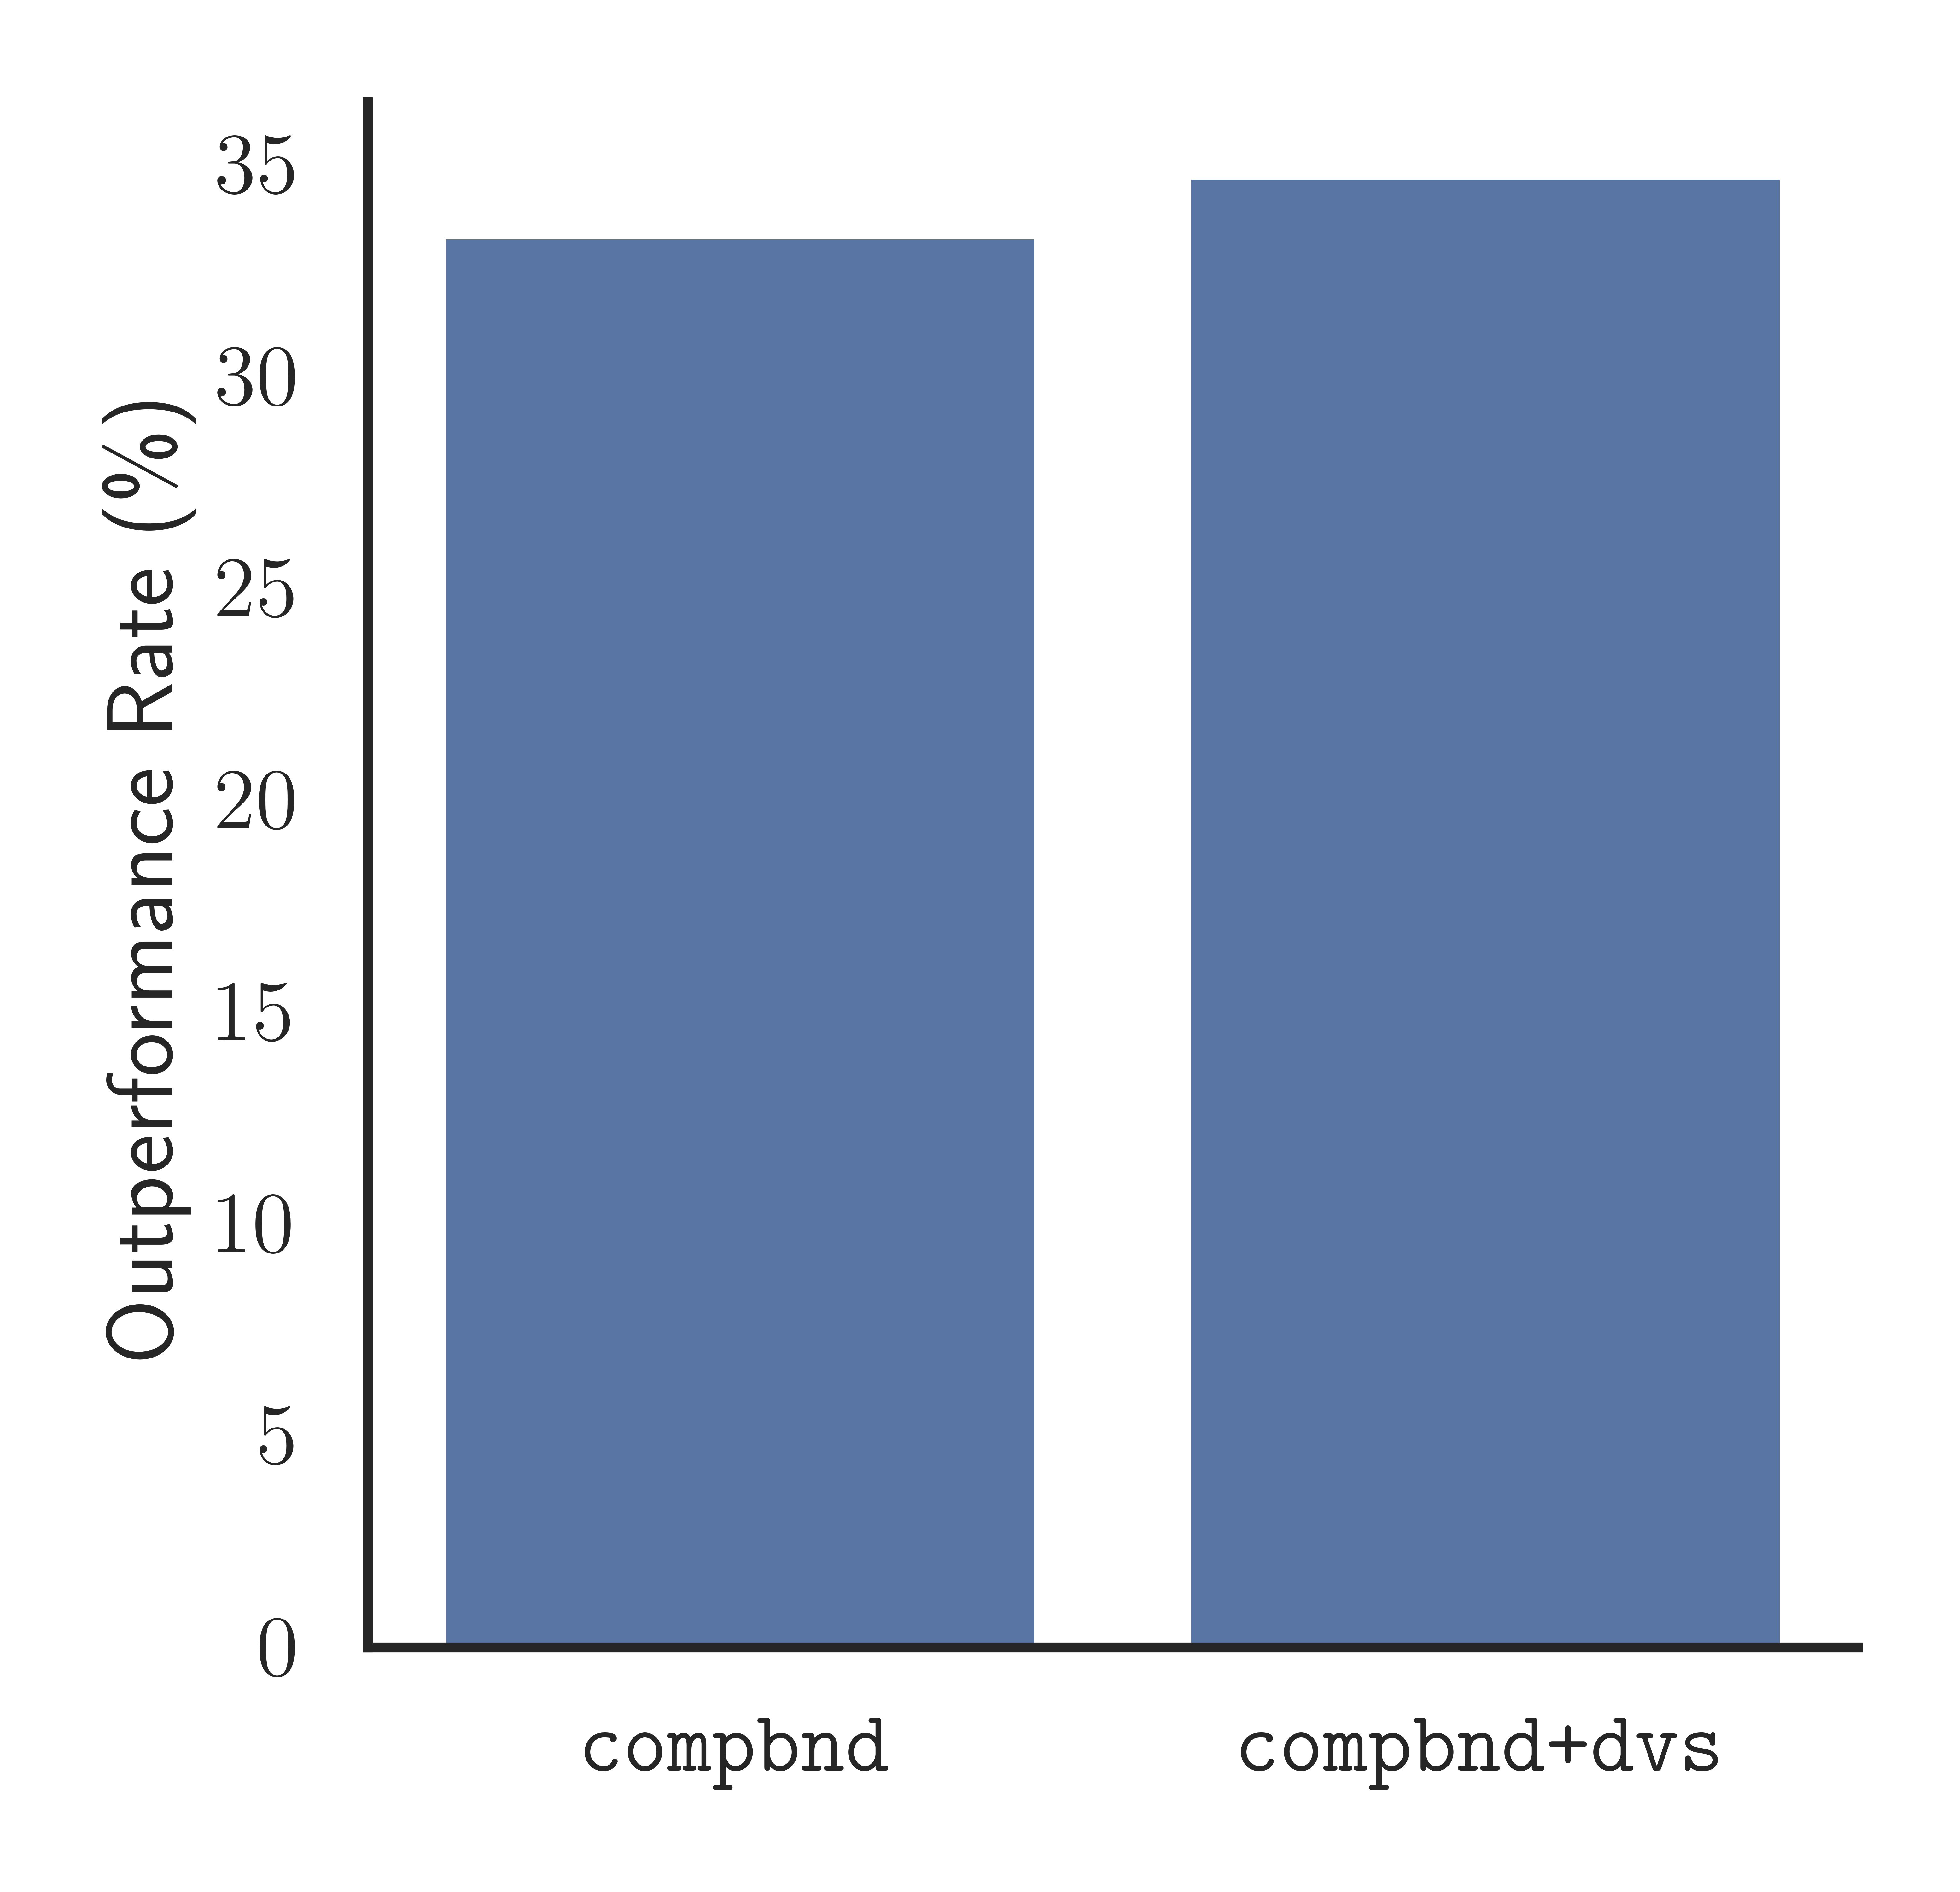
\includegraphics[height=0.85\textheight]{graphics/slides/general/MostFractional/outperforms_generic.png}
\end{figure}
\end{frame}

\begin{frame}
\frametitle{Evaluation $\cdot$ Outperformance Rate over \texttt{generic-mip}}
\centering
\begin{figure}
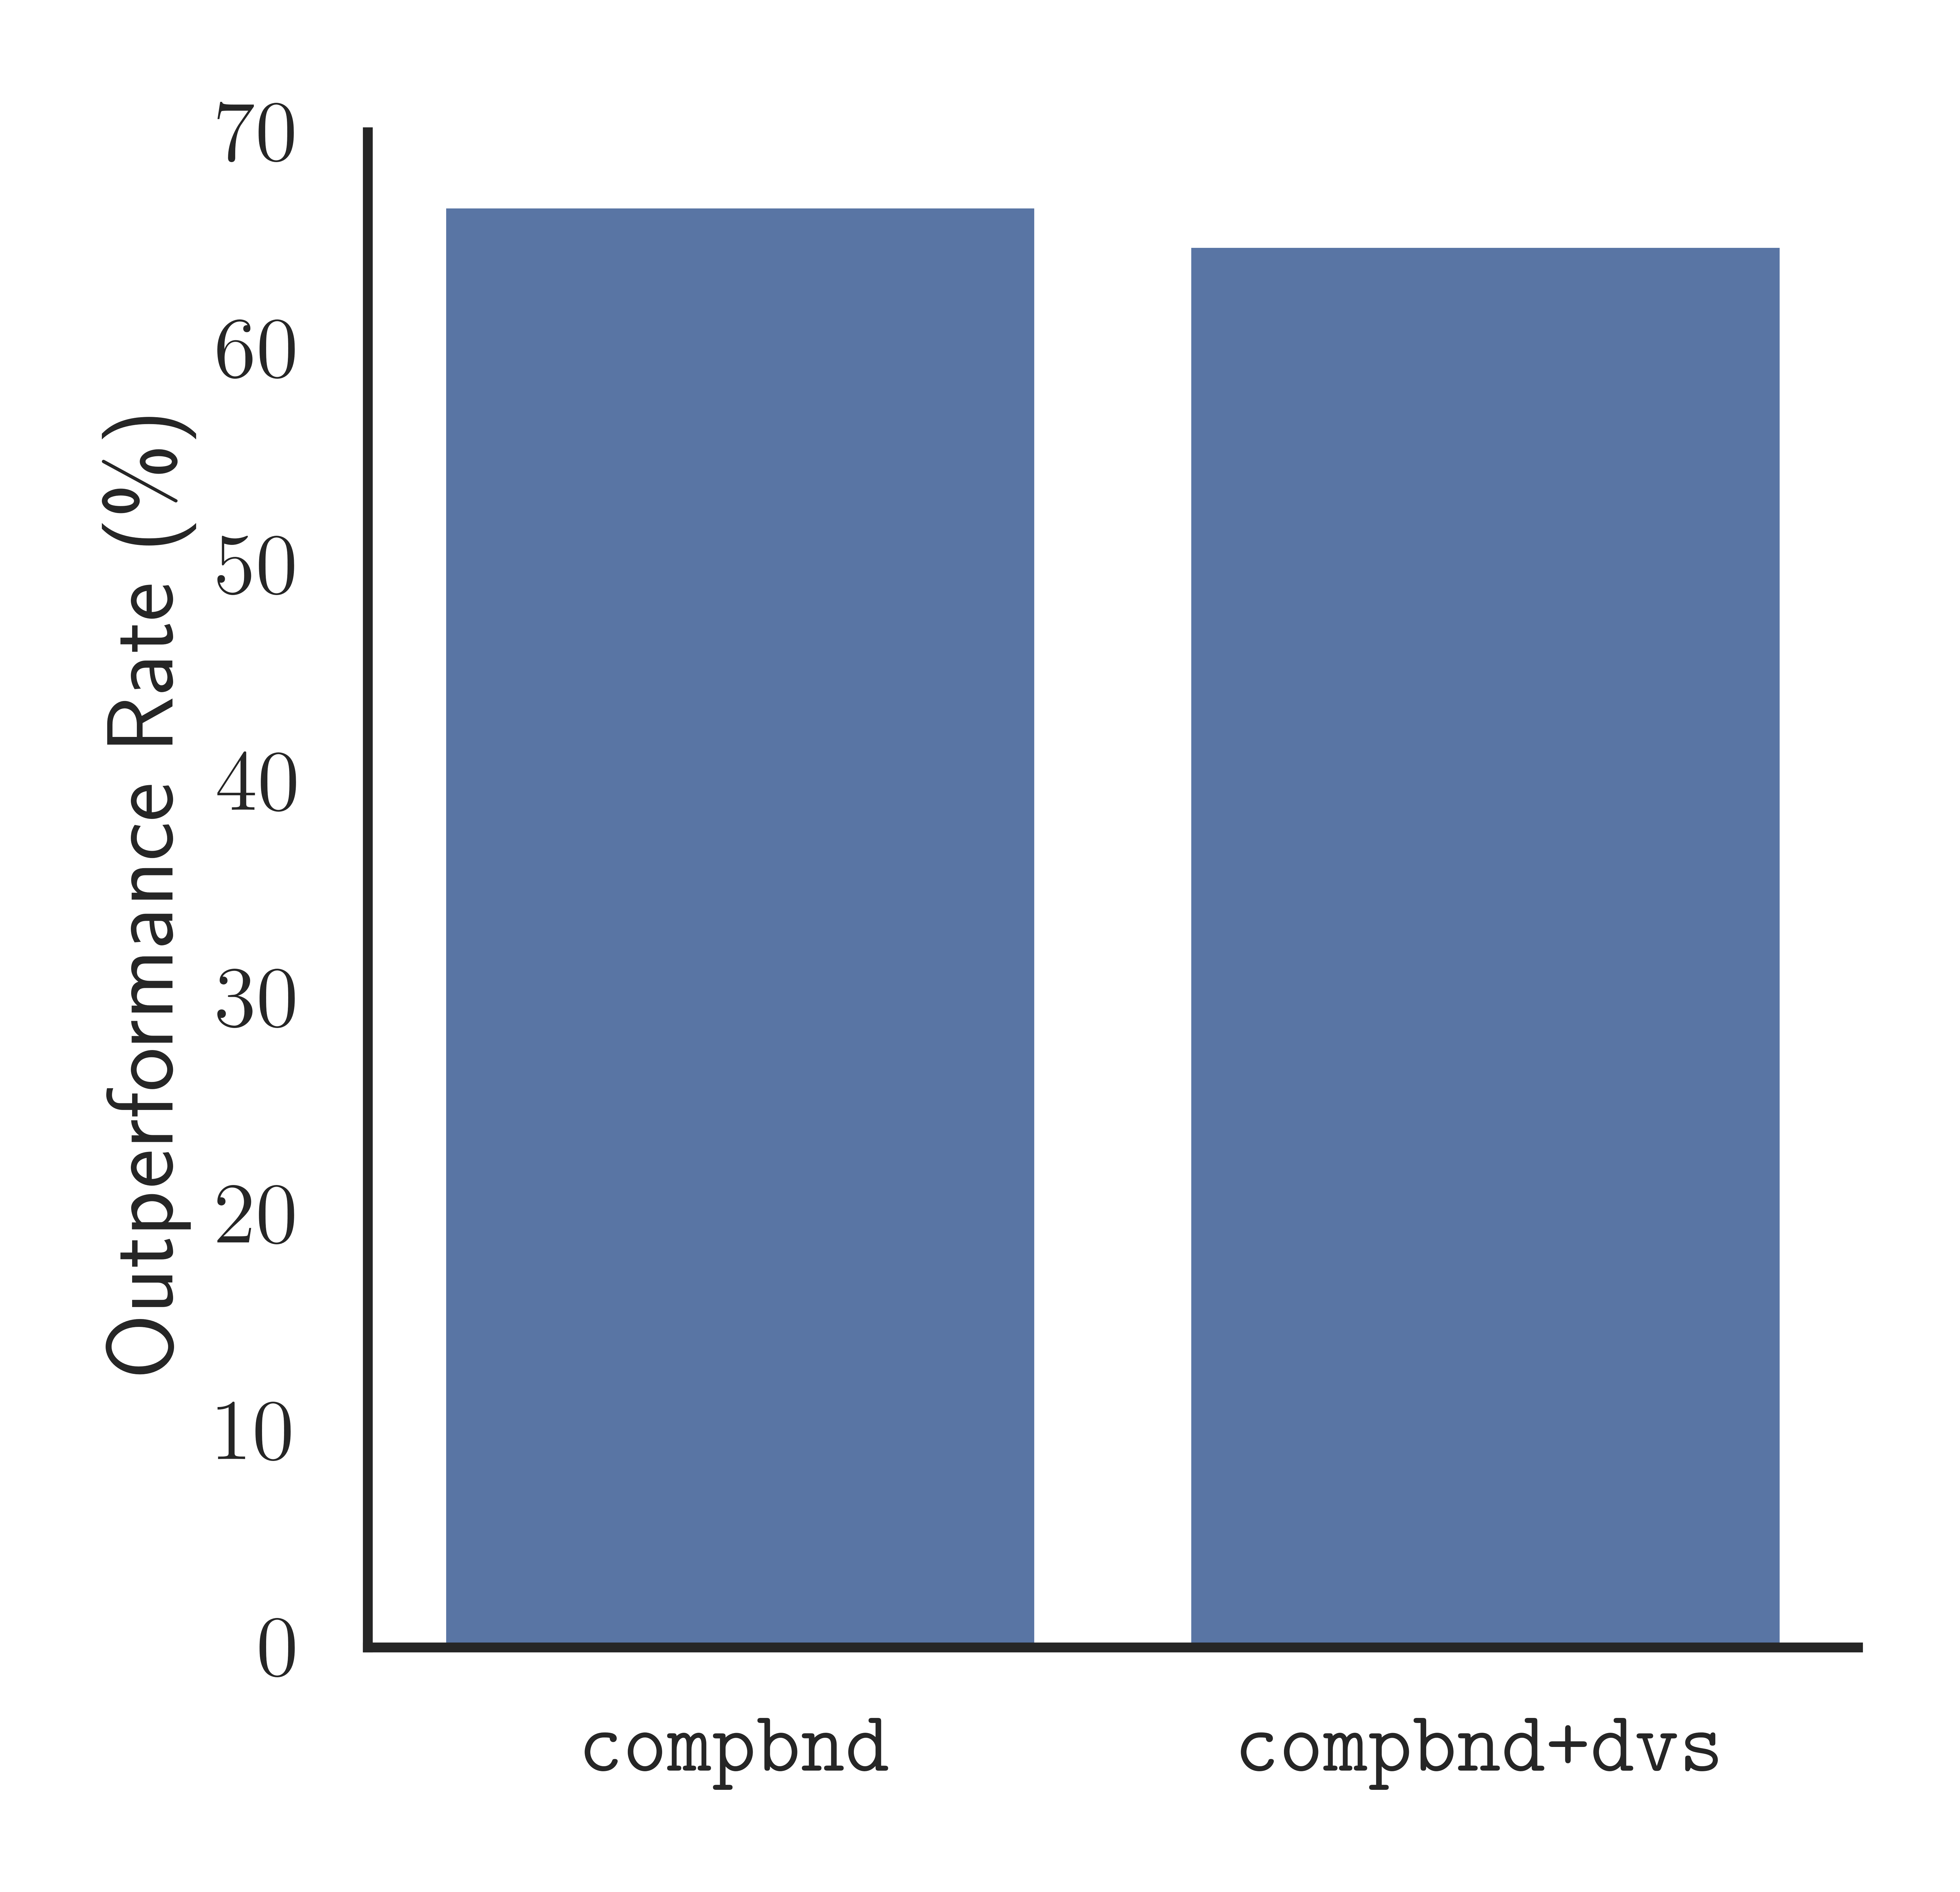
\includegraphics[height=0.85\textheight]{graphics/slides/general/MostFractional/outperforms_generic-mip.png}
\end{figure}
\end{frame}

\begin{frame}
\frametitle{Evaluation $\cdot$ Number of Nodes}
\centering
\begin{figure}
\includegraphics[height=0.85\textheight]{graphics/slides/general/MostFractional/nodes.png}
\end{figure}
\end{frame}

\begin{frame}
\frametitle{Evaluation $\cdot$ Pricing Calls}
\centering
\begin{figure}
\includegraphics[height=0.85\textheight]{graphics/slides/general/MostFractional/pricing_calls.png}
\end{figure}
\end{frame}

\section{Conclusion}

\begin{frame}
\frametitle{Conclusion}

\begin{itemize}
\item	\GCG{} has a {\color{orange} new interface} for generic master constraints
\item	\GCG{} has a {\color{orange} new branching rule} operating on component bound sequences
\item[$\rightarrow$]	opens up new possibilities for future research (e.g., master separators)
\end{itemize}
\end{frame}

\appendix

\begin{frame}
\frametitle{}
\huge Appendix
\centering
\begin{figure}
\includegraphics[height=0.85\textheight]{graphics/slides/general/MostFractional/pricing_vars.png}
\end{figure}
\end{frame}

\begin{frame}
\frametitle{}
\huge Appendix
\centering
\begin{figure}
\includegraphics[height=0.85\textheight]{graphics/slides/bound_stats/num_bounds.png}
\end{figure}
\end{frame}

\begin{frame}
\frametitle{}
\huge Appendix
\centering
\begin{figure}
\includegraphics[height=0.85\textheight]{graphics/slides/bound_stats/avg_num_bounds.png}
\end{figure}
\end{frame}

\begin{frame}
\frametitle{}
\huge Appendix
\centering
\begin{figure}
\includegraphics[height=0.85\textheight]{graphics/slides/bound_stats/compbnd/depths_distribution.png}
\end{figure}
\end{frame}

\begin{frame}
\frametitle{}
\huge Appendix
\centering
\begin{figure}
\includegraphics[height=0.85\textheight]{graphics/slides/bound_stats/compbnd/avg_num_bounds_vs_depth.png}
\end{figure}
\end{frame}

\begin{frame}[allowframebreaks]
\frametitle{References}
\printbibliography[heading=none]
\end{frame}

\end{document}
